\documentclass[12pt, letterpaper]{report}

% Packages
\usepackage[utf8]{inputenc}
\usepackage{geometry}
\usepackage{setspace}
\usepackage{graphicx}
\usepackage{times}
\usepackage{mathptmx}
\usepackage{indentfirst}
\usepackage{amsmath}
\usepackage{lipsum} 
\usepackage{booktabs} 
\usepackage{hyperref}
\usepackage{tablefootnote}
\usepackage{enumitem}
\usepackage{caption}

% Page layout
\geometry{
    top=1in,
    bottom=1in,
    left=1in,
    right=1in,
    includefoot,
    heightrounded,
}

% Line spacing
\doublespacing

% Set paragraph indent
\setlength{\parindent}{0.5in}

\title{\textbf{Housing Price Prediction With Various Models}}
\author{Yinuo Liu 730407898 \\ Zhuoyu Shi 730392737 \\ Shubing Liu 730508266 \\ Yumo Bai 730480742}
\date{\href{https://github.com/YinuoLiu0708/COMP-562-final-project/tree/main}{GitHub Repository Link}}

\begin{document}

\maketitle

\section*{1. Introduction}
Housing price is highly correlated with the welfare of individuals and communities. The fluctuation of housing prices can significantly impact people’s purchasing decisions and investment plans. The variation of housing prices can indicate regional income disparity. There are numerous factors contributing to the ever-changing housing prices, as specific as the square feet and number of bedrooms, and as broad as the economic swing and government policy. How to predict housing prices from existing data is a challenge faced by residents, estate agents, economists, statisticians, and many others. In this report, we will use machine learning methodologies to predict housing prices. 

\section*{2. Data Description}
The dataset used in this analysis was sourced from Kaggle and obtained from the 'House Prices - Advanced Regression Techniques' competition. The link to the data source is \href{https://www.kaggle.com/competitions/house-prices-advanced-regression-techniques/data}{here}. The dataset comprises information related to real estate properties. It consists of 50,000 observations and includes 6 columns: SquareFeet, Bedrooms, Bathrooms, Neighborhood, YearBuilt, and Price. The first 5 features are predictor variables, and the price is the response variable.\vspace{0.75cm}

\begin{tabular}{|p{3cm}||p{3cm}|p{3cm}|p{3cm}|}
\hline
Variable Name &  Variable Type & Mean & SD\\
\hline
SquareFeet & Numerical & 2006.37468 & 575.513241 \\
\hline
Bedrooms & Numerical & 3.49870 & 1.116326 \\
\hline
Bathrooms & Numerical & 3.49870 & 0.815851\\
\hline
Neighborhood & Categorical* & 1.99854 & 0.815838 \\
\hline
YearBuilt & Numerical & 1985.40442 & 20.719377 \\
\hline
Price & Numerical & 224827.32515 &  76141.08154\\
\hline
\end{tabular}

\vspace{0.25cm}
* Neighborhood is converted as: Rural=1, Suburb=2, Urban=3
% \begin{figure}[ht]
%   \centering
%   \begin{minipage}{0.48\textwidth}
%     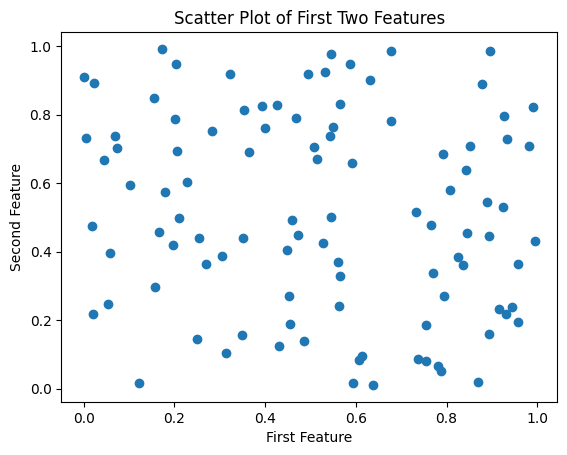
\includegraphics[width=\linewidth]{download-3.png}
%     \caption{Caption for the left image}
%     \label{fig:left_image}
%   \end{minipage}\hfill
%   \begin{minipage}{0.48\textwidth}
%     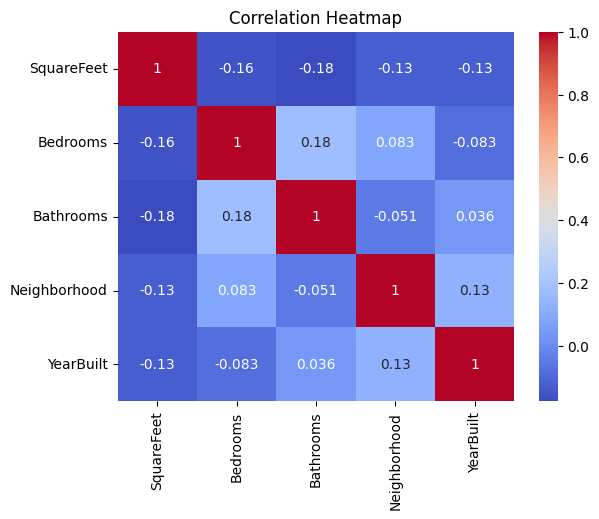
\includegraphics[width=\linewidth]{download-1.png}
%     \caption{Caption for the right image}
%     \label{fig:right_image}
%   \end{minipage}
% \end{figure}
\section*{3. Modeling and Analysis}

We use four regression analysis methods to predict housing prices and compare their accuracy. The methods include Linear Regression, Least Absolute Shrinkage and Selection Operator (LASSO), Random Forest Regression, and Gradient Booster Regressor (GBR). 

\subsection*{3.1 Linear Regression Model Analysis}

The Linear Regression model was chosen as a baseline for the prediction of housing prices. The simplicity of the model makes it a first-line approach in predictive analysis, as it provides a clear interpretation of how each feature influences the target variable – housing prices.

\begin{table}[h]
\centering
\resizebox{\textwidth/(2)}{!}{%
\begin{tabular}{lc}
\toprule
Metric & Value \\
\midrule
Test Mean Square Error (MSE) & \(2.47 \times 10^9\) \\
Test \(R^2\) & 0.573 \\
\bottomrule
\end{tabular}%
}
\caption{Linear Regression model performance}
\end{table}

% Model performance:

% \begin{itemize}[topsep=0pt, partopsep=0pt, parsep=0pt, itemsep=0pt]
%     \item Test Mean Square Error (MSE): 2468771544.275607
%     \item Test $R^2$: 0.5728435816569826
% \end{itemize}

According to the statistics, the $R^2$ score significantly less than 1 suggests that the current model does not adequately capture all the variance in the housing prices, indicating the need for a more complex model or additional features that could better account for the variations in housing prices.

\subsection*{3.2  Least Absolute Shrinkage and Selection Operator}

The Least Absolute Shrinkage and Selection Operator (LASSO) is selected for its advantage in preventing overfitting and performing variable selection. Considering that the features in this dataset may have uneven contributions to the housing price, LASSO serves as a good choice for this housing price prediction task.


% Model performance:

% \begin{itemize} [topsep=0pt, partopsep=0pt, parsep=0pt, itemsep=0pt]
%     \item 5-Fold Cross-Validation MSE: 2492982836.592742 +/- 29111871.97167061
%     \item 5-Fold Cross-Validation $R^2$: 0.5699567726086732 +/- 0.0040731464261042115
%     \item Test MSE: 2468745888.303739
%     \item Test $R^2$: 0.5728480207526445
% \end{itemize}

The LASSO model provides a reasonable fit to the data, explaining 57\% of the variance. Its MSE and $R^2$ values are very close to the baseline model, suggesting that LASSO provides comparable accuracy and explains a similar proportion of the variance to the linear regression. 
\begin{figure}[ht]
  \centering
  \begin{minipage}{0.48\textwidth}
    \centering
    \begin{tabular}{lc}
      \toprule
      Metric & Value \\
      \midrule
      5-Fold Cross-Validation MSE & \(2.43 \times 10^9 \pm 2.92 \times 10^6\) \\
      5-Fold Cross-Validation \(R^2\) & \(0.570 \pm 0.004\) \\
      Test MSE & \(2.47 \times 10^9\) \\
      Test \(R^2\) & 0.573 \\
      \bottomrule
    % \caption{LASSO model performance}
    \end{tabular}
    \captionof{table}{LASSO model performance}
    \label{tab:lasso_performance}
  \end{minipage}\hfill
  \begin{minipage}{0.38\textwidth}
    \centering
    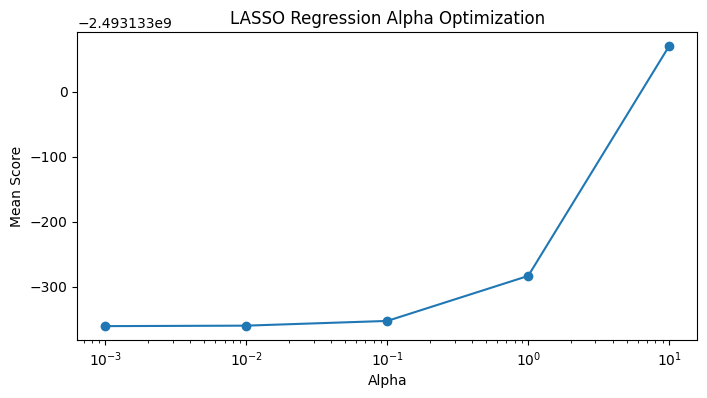
\includegraphics[width=\linewidth]{download-4.png}
    \caption{LASSO Regression Alpha Optimization}
    \label{fig:second_image}
  \end{minipage}
\end{figure}
% \begin{table}[h]
% \centering
% \begin{tabular}{lc}
% \toprule
% Metric & Value \\
% \midrule
% 5-Fold Cross-Validation MSE & \(2.43 \times 10^9 \pm 2.92 \times 10^6\) \\
% 5-Fold Cross-Validation \(R^2\) & \(0.570 \pm 0.004\) \\
% Test MSE & \(2.47 \times 10^9\) \\
% Test \(R^2\) & 0.573 \\
% \bottomrule
% \end{tabular}
% \caption{LASSO model performance}
% \end{table}

% \begin{figure}[ht]
%   \centering
%   \begin{minipage}{0.48\textwidth}
%     \centering
%     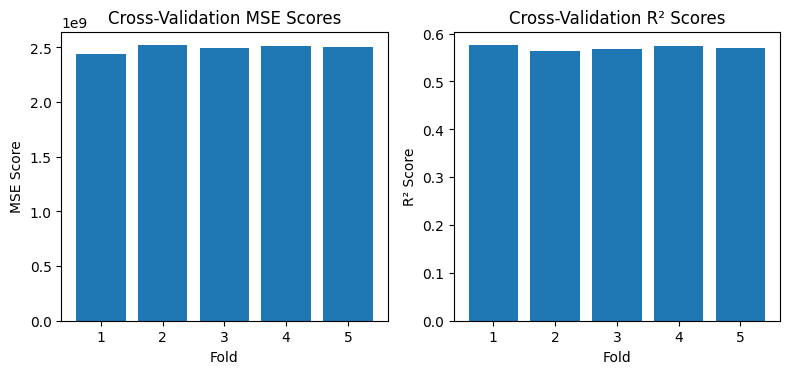
\includegraphics[width=\linewidth]{download-5.png}
%     \caption{Caption for the first image}
%     \label{fig:first_image}
%   \end{minipage}\hfill
%   \begin{minipage}{0.48\textwidth}
%     \centering
%     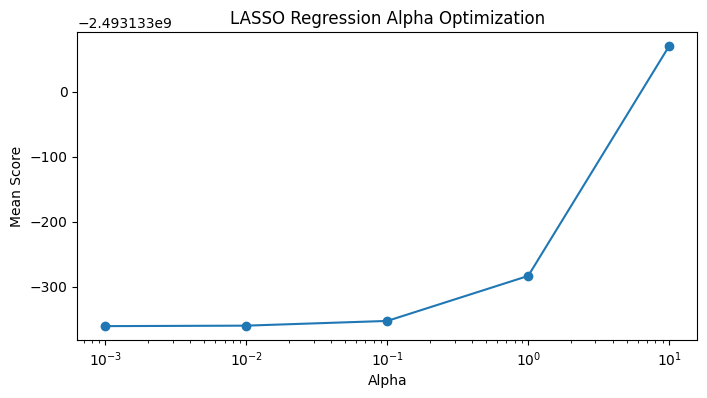
\includegraphics[width=\linewidth]{download-4.png}
%     \caption{Caption for the second image}
%     \label{fig:second_image}
%   \end{minipage}
% \end{figure}
\vspace{-0.55cm}
\subsection*{3.3 Random Forest}

Random forest is selected for its resistance against noise and outliers in the data. It's a supervised learning algorithm that combines the predictions of multiple decision trees to reduce overfitting and improve accuracy. 
\begin{table}[h]
\centering
\resizebox{\textwidth/(2)}{!}{%
\begin{tabular}{lc}
\toprule
Metric & Value \\
\midrule
5-Fold Cross-Validation MSE & \(2.53 \times 10^9 \pm 2.72 \times 10^7\) \\
5-Fold Cross-Validation \(R^2\) & \(0.564 \pm 0.0037\) \\
Test MSE & \(2.53 \times 10^9\) \\
Test \(R^2\) & 0.564 \\
\bottomrule
\end{tabular}%
}
\caption{Random Forest Performance}
\end{table}


% Model performance:

% \begin{itemize}[topsep=0pt, partopsep=0pt, parsep=0pt, itemsep=0pt]
%     \item 5-Fold Cross-Validation MSE: 2526867451.760862 +/- 27138793.35331006
%     \item 5-Fold Cross-Validation $R^2$: 0.5641104831619396 +/- 0.0037409341851049856
%     \item Test MSE: 2532594262.239625
%     \item Test $R^2$: 0.5639290760524656
% \end{itemize}

The random forest model explains about 56\% of the variance in test data. It has similarly good performance in predicting housing prices as linear regression and LASSO. 


\subsection*{3.4 Gradient Boosting Regressor Model}

The Gradient Boosting Regressor (GBR) was selected due to its robustness and effectiveness in handling various types of data distributions. It can capture intricate patterns in the data, making it a preferred choice for the housing price prediction task where such complexities are common due to the multifaceted nature of real estate markets.
% \begin{table}[h]
% \centering
% \begin{tabular}{lc}
% \toprule
% Metric & Value \\
% \midrule
% 5-Fold Cross-Validation MSE & \(1.06 \times 10^{11} \pm 1.60 \times 10^{10}\) \\
% 5-Fold Cross-Validation \(R^2\) & \(-0.2466 \pm 0.3014\) \\
% Test MSE & \(1.01 \times 10^{11}\) \\
% Test \(R^2\) & \(-0.1775\) \\
% \bottomrule
% \end{tabular}
% \caption{GBR performance}
% \end{table}
\begin{table}[h]
  \centering
  \resizebox{\textwidth/(2)}{!}{%
    \begin{tabular}{lc}
      \toprule
      Metric & Value \\
      \midrule
      5-Fold Cross-Validation MSE & \(1.06 \times 10^{11}\) \\
      5-Fold Cross-Validation \(R^2\) & \(-0.2466 \pm 0.3014\) \\
      Test MSE & \(1.01 \times 10^{11}\) \\
      Test \(R^2\) & \(-0.1775\) \\
      \bottomrule
    \end{tabular}%
  }
  \caption{GBR performance}
\end{table}

% Model performance:

% \begin{itemize}[topsep=0pt, partopsep=0pt, parsep=0pt, itemsep=0pt]
%     \item 5-Fold Cross-Validation MSE: 106,119,777,257.88 +/- 15,981,507,525.53
%     \item 5-Fold Cross-Validation $R^2$: -0.2466 +/- 0.3014
%     \item Test MSE: 100,754,861,599.48
%     \item Test $R^2$: -0.1775
% \end{itemize}

The negative $R^2$ scores from both cross-validation and testing imply that the current GBR model does not provide a reliable prediction for housing prices. The high variability in MSE across the folds also suggests that the model's performance is inconsistent.
\vspace{-0.55cm}
\section*{4. Discussion}
In the data analysis, Linear Regression, LASSO, and Random Forest explain similar percentages of variance in the train and test data with comparable accuracy. The consistency in the three models’ performance suggests that the relationships between the predictor variables and the response variable are predominantly linear. Therefore, methods that explicitly model linear relationships perform similarly well or even better than complex models. The Gradient Boosting Regressor model, on the other hand, does not reliably predict housing prices evidenced by its negative $R^2$ and high variability in MSE. Its poor performance could be attributed to GBR’s difficulty in capturing linear relationships as the model is designed for non-linear relationships in the data. 

The model with the best performance on test data, LASSO, explains approximately 57.28\% of the variance of housing prices, which suggests a moderate fit of the model to the data. The limitation of model performance could be attributed to the number of features and observations included in the dataset. The five predictor features used in the analysis fail to account for a large portion of the variance in housing prices. For future improvements, including more features like locations might contribute to more accurate predictions of housing prices.

% Using a recent dataset with more observations could also potentially enhance the model performance.  

\end{document}
